%!TEX TS-options = -shell-escape
\documentclass[oribibl]{llncs}
\pagestyle{headings}
\usepackage{natbib}
\usepackage{todonotes}
\bibliographystyle{alpha}
\newenvironment{changemargin}[2]{
\begin{list}{}{
\setlength{\topsep}{0pt}
\setlength{\leftmargin}{#1}
\setlength{\rightmargin}{#2}
\setlength{\listparindent}{\parindent}
\setlength{\itemindent}{\parindent}
\setlength{\parsep}{\parskip}
}
\item[]}{\end{list}}
\usepackage{url}
\usepackage{listings}
\usepackage{pdfpages}

\lstdefinelanguage{scala}{
  morekeywords={abstract,case,catch,class,def,%
    do,else,extends,false,final,finally,%
    for,if,implicit,import,match,mixin,%
    new,null,object,override,package,%
    private,protected,requires,return,sealed,%
    super,this,throw,trait,true,try,%
    type,val,var,while,with,yield},
  otherkeywords={=>,<-,<\%,<:,>:,\#,@},
  sensitive=true,
  morecomment=[l]{//},
  morecomment=[n]{/*}{*/},
  morestring=[b]",
  morestring=[b]',
  morestring=[b]"""
}

\usepackage{alltt}
\usepackage{pgfplots}
\usepackage{graphicx}

\begin{document}
\mainmatter{}
\title{Work-stealing Queues In Practice}
\author{Sune Alk\ae{}rsig, Thomas Hallier Didriksen, and Christian Harrington \\
\email{\{sual, thdi, cnha\}@itu.dk}}

\institute{IT University of Copenhagen, Rued Langgaards Vej 7, 2300 Copenhagen S, Denmark}
\maketitle

\begin{abstract}
There are many solutions for scheduling work across multiple threads, one of which is the work-stealing queue. 
In this paper we examine several implementations of work-stealing queues, such as the one described by Arora, Blumofe, and Plaxton, as well as several queues for idempotent work.
We have implemented these queues for the Java Virtual Machine, and we benchmark them using four test cases, to be able to compare their relative performance.
Our findings show that the simple Arora, Blumofe, and Plaxton queue is very competitive compared to later extensions.
We also find that the idempotent queues' performance is greatly dependent on the task at hand, more so than the other implementations.

\keywords{Work-stealing queues}
\end{abstract}

%!TEX root = ../Work-stealing Queues.tex
\section{Introduction}
\label{sec:introduction}
A popular way of scheduling parallel workloads across multiple threads is
through use of the work-stealing queue. Several different variations of the
work-stealing queue exists, featuring different advantages and drawbacks. In
this report we describe 6 different queue varieties, in order to present an
overview of the different approaches available when implementing a
work-stealing queue. We have also implemented these queues in the Scala
programming language, along with several different cases that use them. This is
done in order to compare the performance of the different queues in different
situations. 

This report is structured as follows: In Section~\ref{sec:background}, we cover
the necessary background, covering different approaches to concurrency, as well
as work-stealing queues themselves. In Section~\ref{sec:implementations} we
describe the six different queues we have implemented, along with their
differences. Section~\ref{sec:benchmarks} describes the different cases we have
implemented, along with our benchmarking results for each case. An analysis of
these results are presented in Section~\ref{sec:performance_analysis}. Our
testing approach is explained in Section~\ref{sec:testing}, while we reflect
on the project in Section~\ref{sec:Reflection}. We conclude in 
Section~\ref{sec:conclusion}.

%!TEX root = ../Work-stealing Queues.tex
\section{Background}
\label{sec:background}

This section presents the concepts underlying the queue implementations and the subsequent analysis. In particular, different approaches to creating concurrent application are discussed.

\subsection{Common Concurrency Problems}
Many errors can arise which are directly caused by the presence of concurrent computations. One of the most important problems related to work-stealing queues is the \emph{ABA problem}. This problem can occur in the context of a \emph{compare-and-swap} operation, where the update is performed if the value of the given register is as expected. However, this provides no guarantees that the value has not changed since we last observed it, and then been changed back by another thread. Thus, the ABA problem gets its name from the notion that the register was \emph{A} when we observed it, but then changed to \emph{B} and back to \emph{A} before our next observation. In some situations we need to prevent this from happening, which may require specific measures to be taken.

Another common problem is \emph{check-then-act}. This problem can arise if a thread is supposed to perform some action as a consequence of the successful result of a check. If the thread first performs the check successfully, but is then suspended by the scheduler, then the result of the check might no longer be valid when the thread is later resumed, since other threads could have made changes to the shared state in the meantime. In such case, the invariants of the system could be violated if the planned action is performed by the resumed thread.

\subsection{Approaches to Concurrency}
The complexity of building concurrent applications arises mostly from the inherent need to manage concurrent access to shared state, in particular shared \emph{mutable} state. With shared mutable state, any thread may write to any memory location at any time (in principle), which makes maintaining the invariants of the system a major concern. Keeping shared state immutable eliminates many such problems, as no threads will ever read different data from the same memory location at different moments in time. While it is arguably easier to reason about concurrent applications with immutable shared state, having mutable state can be desirable for several reasons, the most compelling of which is (possible) increased performance. In the following, we will discuss different approaches to handling concurrent access to shared mutable state.

% locks
\subsubsection{Lock-based Synchronization}
Locking is a widely used mechanism for handling access to shared mutable state, especially in the realm of imperative programming. Locks can be used to grant exclusive access to one or more shared resources by associating that resource with a lock (assuming a locking scheme with \emph{mutual exclusion locks}, where a given lock can only be held by one thread at a given point in time). The problem of synchronization is solved by a guarantee that no other threads will be accessing the shared resource as long as the lock is being held. Since any access to the resource must be exclusive, a lock must be obtained both when reading from and writing to it. 

While the exclusive locking mechanism preserves the integrity of the shared state, this exclusivity is also one of the greatest disadvantages of locking. Whenever a thread tries to obtain a lock held by another thread, the call blocks and the thread is suspended and must wait (potentially forever) for the current lock owner to finish its work. During this time, the waiting thread cannot do anything else. For locks under high contention, the performance degradation caused by the overhead of suspending and resuming threads might be very high, especially if the lock is only required for reading. For these situations, the use of non-blocking synchronization can be preferable.


% blocking vs. non-blocking queues
\subsubsection{Non-blocking Synchronization}
Instead of taking the pessimistic approach of making sure that exclusive access is obtained before performing any operations on a shared resource, non-blocking synchronization is more optimistic in nature\,\citep{Goetz2006}. Being \emph{non-blocking} means that if a thread fails or is suspended, it cannot cause another thread to fail or be suspended, because threads accessing a shared resource never have to wait for another thread (contrary to the lock-based scheme, where a thread may have to wait for the release of a lock)\,\citep{Goetz2006}. A non-blocking algorithm can be said to be \emph{lock-free}, which means that at any point of execution, some thread is making progress (and thus the term has nothing to do with lock-based synchronization).

In the non-blocking scheme, the integrity of a shared resource is ensured by only allowing updates to happen atomically from a consistent state, where all the invariants of the system hold. If some invariant does not hold, e.g. when a shared variable has another value than expected because it has been updated by another thread, a recovery mechanism is triggered instead. To perform atomic non-blocking updates, specific processor instructions (e.g. compare-and-swap) must be used to avoid common concurrency problems such as \emph{check-then-act}. 

Non-blocking synchronization provides a more fine-grained approach to synchronization, where the cost of suspending and resuming threads is replaced by the need for a recovery mechanism when faced with failed updates (retrying is a perfectly valid recovery mechanism). However, a non-blocking algorithm can be more complicated to design than a similar lock-based one\,\citep{Goetz2006}, so using non-blocking synchronization might not always be desirable.

% Here, specific processor instructions (e.g. \emph{compare-and-swap}) are used to perform atomic compound operations on shared resources, but in contrast 

% Non-blocking synchronization utilizes hardware support to ensure the integrity of shared state. Instead of using locks to perform atomic compound operations, specific processor instructions, such as \emph{compare-and-swap}, are used to make sure that updates to shared resources only happen from a consistent state. As opposed to exclusive locking, non-blocking operat

% As opposed to the pessimistic approach of locking, where all locks must be obtained before 
% lock-free vs. wait-free ?

\subsection{A Simple Solution}
The simplest solution to the problem of concurrently processing \emph{n} suspended computations (denoted ``work units'' or simply ``work''), is to have \emph{m} worker threads processing these in parallel from a central queue. To avoid two threads handling the same work unit, a lock is placed on this central queue, which must be held in order for a thread to take more work. Whenever two or more threads finish their current work simultaneously, they will all try to obtain the lock from the queue. However, only one of them will succeed, and the others will be suspended while waiting for the lock. In these situations, many threads will be idle at any given time when contention for the lock gets high. Consequently, this design leads to a situation where the central work queue becomes a bottleneck, and computational resources are wasted while threads are idle. Although not very efficient, a simple design such as this can serve as a good baseline for comparison with other approaches.


\subsection{Work-stealing Queues} % What is a work-stealing queue?
A work-stealing queue is a queue implementation that facilitates working with work-stealing scheduling algorithms\,\citep{Arora:1998:TSM:277651.277678}. In a work-stealing scheduling algorithm, each thread is assigned a work-stealing queue, the elements of which are work units. This queue has the standard \texttt{push} and \texttt{take} operations for adding and removing elements from it, respectively, and only the thread owning the queue has access to these operations. Additionally, the queue exposes a \texttt{steal} operation, through which other threads may ``steal work''. An example of such a scenario is shown in Figure~\ref{fig:workstealing_scenario}.

Work-stealing algorithms are especially well-suited for solving problems where one unit of work may generate more work (examples of which can be found in Section \ref{sec:benchmarks}). The idea is that whenever the work unit processed by a given thread generates more work, this work is stored in the thread's local queue. When the thread finishes its current work, it first examines its own queue, and continues to process any work it might find. If no work is found locally, the thread begins to examine the queues of other threads, in effect ``stealing'' the work generated by these. This design leads to efficient utilization of computation resources, since a thread is never idle: it is either working or looking for more work.

\begin{figure}
\begin{center}
\includegraphics[scale=1]{resources/WSQ.pdf}
\end{center}
\caption{An example situation from a work-stealing algorithm with four working threads. Each thread has its own queue. Thread 3 has completed all of its own work, and is therefore in the process of stealing work from thread 4.}
\label{fig:workstealing_scenario}
\end{figure}

\subsection{Software Transactional Memory}
Software Transactional Memory (STM) is an attempt to address the difficulty of designing concurrent algorithms and data structures, by enabling the user to specify concurrent operations as transactions. Following the formulation of transactional memory presented by Herlihy and Moss\,\citep{HerlihyMossTM}, Shavit and Touitou proposed the first model for software-only transactional memory\,\citep{ShavitSTM}. Using STM, shared memory can be accessed and updated by means of transactions, where a transaction is understood as an application of a finite sequence of primitive operations to that shared memory. Furthermore, the transactions must have the properties of \emph{atomicity} (transactions appear to happen sequentially) and \emph{serializability} (the sequential order of transactions is consistent with their real-time order)\,\cite{ShavitSTM}.

Ideally, designing concurrent algorithm with STM should shift much of the burden of worrying about concurrency from the user to the runtime system, without incurring any performance trade-offs. A study done by Dice and Shavit\,\citep{Dice06whatreally} shows that algorithms implemented using STM scale better than equivalent hand-crafted algorithms, both lock-based and non-blocking. However, opponents of STM claim that it causes a higher sequential overhead than more traditional shared-memory approaches\,\citep{Cascaval08}, since transactions expand to many more load and store instructions, leading to performance losses.

In an improvement to their earlier algorithm, Dice, Shalev, and Shavit\,\citep{DiceTLII} present the \emph{Transactional Locking II} algorithm, which supposedly is ``an order of magnitude faster than sequential code made concurrent using a single lock.'' This is achieved using a global version-clock, which allows for fast read-only transactions. Although these findings seem promising, the debate concerning the performance of concurrent algorithms implemented using STM has yet to reach consensus.

%!TEX root = ../Work-stealing Queues.tex
\section{Implementations}
\label{sec:implementations}
In the following section we will describe the work-stealing queues we have implemented. Upon each queue three operations can be made, two of which are classic queue operations. The \texttt{push} operation simply adds a task to the queue and \texttt{take} removes a task from the queue. These operations are only meant to be used by the owner of the queue. The third operation, \texttt{steal}, allows threads to ``steal'' work from other threads. While the \texttt{steal} and \texttt{take} operations have similar effects, they have to work differently to ensure the consistency of the queue.

\subsection{Arora-Blumofe-Plaxton (ABP) Queue}
The ABP queue\,\cite{Arora:1998:TSM:277651.277678} holds its tasks in an array and uses \texttt{top} and \texttt{bottom} pointer to keep track of the start and end of the queue. Pushing a task to the queue (\texttt{push}) is straightforward. Just add it to the array at the \texttt{bottom} position and increment \texttt{bottom}. Taking tasks from the queue requires more work to ensure that the same work is not extracted twice as \texttt{take} and multiple different \texttt{steal} operations can happen simultaneously. Avoid duplication is done by only allowing \texttt{steal} to return if the \texttt{top} has remained unchanged throughout the operation. This, however, is not sufficient\,\cite[p. 4]{Arora:1998:TSM:277651.277678} as it is still prone to the ABA problem. If the queue is emptied and refilled to the same size between the read from the queue (Figure \ref{fig:abpsteal} line 9) and the comparison with \texttt{top} (Figure \ref{fig:abpsteal} line 12) the read might no longer be valid. To handle this a \texttt{tag} value is added, which is incremented whenever the queue is completely emptied. This \texttt{tag} together with \texttt{top} is now known as \texttt{age}. Now, instead of just the \texttt{top} having to remain unchanged, the entire \texttt{age} must be the same.

\begin{figure}
\begin{lstlisting}[language=scala,basicstyle=\ttfamily\bfseries\scriptsize,numbers=left]
final def steal(): Option[E] = {
    val oldAge = age.get
    val localBot = bottom

    if (localBot <= oldAge.top) { // Queue is Empty
      None
    }
    else {
      val v = queue.get(oldAge.top)
      val newAge = Age(oldAge.tag, oldAge.top + 1)

      if (age.compareAndSet(oldAge, newAge)) { 
      	// CAS for ABA prevention
        Some(v)
      }
      else {
        None
      }
    }
  }
\end{lstlisting}
\caption{ABP implementation of \texttt{steal}.}
\label{fig:abpsteal}
\end{figure}

\subsection{Chase-Lev Queue}
Chase and Lev designed an improved version of the ABP queue using circular arrays\,\citep{ChaseLev05}. The Chase-Lev implementation solves the fundamental problem from which the ABP queue suffers, namely the use of fixed-size arrays. Fixed-size arrays make the ABP queue prone to overflow problems, while also leading to inefficient memory usage: In a system with \emph{n} threads and allocated memory \emph{m}, any queue in the system can hold at most $\frac{m}{n}$ elements. Using dynamic circular arrays, any Chase-Lev queue can be grown when necessary, which means that the shared memory does not have to be divided among the queues upfront. To improve memory usage, Chase and Lev also describe a shrinking operation for the underlying circular arrays, such that memory is reclaimed whenever the actual size of an array is less than the allocated size by some constant factor. Since the \texttt{top} pointer is never decremented, the size of a given Chase-Lev queue is only restricted to the size of \texttt{top} (Chase and Lev use a 64-bit integer). Contrary to the ABP queue, the Chase-Lev implementation does not need a tag to avoid the ABA problem. As a direct consequence of the \texttt{top} pointer never being decremented, any thread will always notice if the contents of the queue have changed (using a \emph{compare-and-swap} operation on \texttt{top}).

While all our tests have been run in a garbage-collected environment on the JVM, the Chase-Lev queue does not rely on garbage collection for memory management.

\subsection{Idempotent Queues}
The previously discussed queues guarantee that no task will be extracted twice. This strictness can be relaxed in some cases to possibly improve performance\,\cite[p. 46]{Michael:2009:IWS:1594835.1504186}. The rest of the queues don't have this guarantee, which means that they can only be used in cases where this idempotence does not violate the semantics of the tasks. As such these queues can only be used for cases where it is allowed to execute the same task twice.

We have implemented three different approaches to idempotent work stealing\,\cite{Michael:2009:IWS:1594835.1504186}. Generally, all three work in similar fashion, but the order in which tasks are extracted differ from queue to queue. All three queues keep their tasks in an array, but uses different ways of keeping track of the ends of the queue. When talking about these queues we use the term ``queue'' loosely to mean a data structure that keeps its elements in order.

\paragraph{The Idempotent LIFO}\,\cite[p. 47]{Michael:2009:IWS:1594835.1504186} does not need to track where the queue starts as tasks are always added to, and extracted from the end. The end of the queue is simply noted by a \texttt{tail} pointer indicating the end. The \texttt{tail} points to the last task in the queue, and if it is zero the queue is empty. This \texttt{tail} is packed with a \texttt{tag} in an \texttt{anchor} for ABA prevention when stealing. This \texttt{anchor} must remain unchanged between the read of a stolen value and the return of this value. It is worth noting that, in contrast to the other queues, this queue (along side the Idempotent FIFO queue) \texttt{steal} and \texttt{take} from the same end of the queue.

\paragraph{The Idempotent FIFO}\,\cite[p. 48]{Michael:2009:IWS:1594835.1504186}  adds tasks to the beginning of the queue and extracts (both \texttt{steal} and \texttt{take}) from the end of the queue. Therefore it needs to track both the start (\texttt{head}) and the end (\texttt{tail}) of the queue. Interestingly enough this implementation does not need ABA prevention as tasks are always added to a different end than they are taken.

\paragraph{The Idempotent Double-Ended} \,\cite[p. 49]{Michael:2009:IWS:1594835.1504186} adds and steals tasks from the beginning of the queue and takes tasks from the end. This means that this implementation also needs ABA prevention. This is done a similar way as the LIFO with a \texttt{anchor} packed with the \texttt{head}, \texttt{size}, and a \texttt{tag} .

\subsection{Duplicating Queue}
Similar to the idempotent queues the duplicating queue\,\cite[p. 233]{Leijen:2009:DTP:1639949.1640106} can potentially return a pushed task more than once. When stealing from this queue the stolen task is either removed from the queue or just duplicated. When a task is the only element in the queue both \texttt{steal} (going from the \texttt{head}) and \texttt{take} (going from the \texttt{tail}) will access the same task. In this case we say that the task has been ``duplicated''. Two thieves cannot steal the same element from the queue as stealing requires a lock.

Furthermore, if a new element is pushed just after the above duplication, the \texttt{head} and \texttt{tail} pointers are inconsistent\,\cite[p. 235]{Leijen:2009:DTP:1639949.1640106}. This is solved by another pointer \texttt{tailMin} indicating the minimal index at which a task has been taken. When checking if the queue is empty when taking, \texttt{head} is compared to the smallest value of \texttt{tailMin} and \texttt{tail}.

\subsection{Comparison}
Our implementations can be split into two categories: Those that are idempotent, and those that are not. The idea behind the idempotent queues is that the queue operations themselves are simpler, but at the risk of performing the same task multiple times. This means that we can expect the idempotent queues to perform well in cases where there are many queue operations. They will, however, not work in cases where the same work is not allowed to be done twice. For us this means that the queues that are idempotent cannot be tested on our quick sort and XML serialization cases.

Amongst the idempotent queues the duplicating queue stands out. Since it is only idempotent when the owner and exactly one thief attempts to access a queue with exactly one element, duplication of work is a lot more seldom. This comes at the cost of only allowing one thief to steal from the same queue at ones which will slow down stealing.

The non-idempotent queues are the ABP and Chase-Lev queues. They are very similar, but the key difference is that the size of ABP is fixed where as Chase-Lev can grow. This means that ABP is more memory intensive, but should perform better than Chase-Lev as it does not need to grow the queue. We have also made an implementation of Chase-Lev that also shrinks the queue which should be even more memory efficient at the cost of performance.

%!TEX root = ../Work-stealing Queues.tex
\section{Benchmarks}
To test our different queue implementations, we developed a small framework
for parallelizing computations using work-stealing queues. There are three
main components, the \texttt{WorkerPool}, \texttt{Worker}, and \texttt{Node}
traits. For each of the cases below, classes implementing these traits were
created. The \texttt{WorkerPool} is in charge of starting the desired number
of threads, and assigning each \texttt{Worker} to a thread. The \texttt{Worker}
holds a queue, and contains the main logic for the case. \texttt{Node}s
represent individual ``work units'', and are the elements contained in the
queues.

\label{sec:benchmarks}
\subsection{Cases}
To test our different work-stealing queues, we have implemented four different
examples.
\subsubsection{Raw Queue Operations} %Raw

The first, which we call ``Raw'', is meant to do as little work as possible,
and thus to stress the queue implementations as much as possible. A
\texttt{RawTreeBuilder} builds a tree of \texttt{Node}s, which hold an
arbitrary number of children, and nothing else. Each \texttt{Worker} simply
looks at a \texttt{Node}, and adds all its children to the queue, before
moving to the next \texttt{Node}. This means that queue operations will be the
deciding factor for how long a run will take. It should be noted that this is
an unrealistic workload, as no actual work is done, besides traversing the
tree.

\subsubsection{Quick Sort} % Quick sort
Our second case is a simple quick sort implementation. It is simple in that it
does not sort in-place. Instead, when splitting an array, each new child
\texttt{Node} receives a full copy of the array to split. When a lower
threshold for array length is reached, insertion sort is used. Once an array
has been sorted using insertion sort, its parent \texttt{Node} is notified. If
both the parent \texttt{Node}'s children have been sorted, the parent
\texttt{Node} is added to the queue. When the parent \texttt{Node} is examined
by a \texttt{Worker}, the two sorted subarrays are combined, and the next
parent \texttt{Node} in the hierarchy is notified. When both children of the
root \texttt{Node} are combined, the entire array has been sorted.

\subsubsection{Spanning Tree} % Spanning tree
For our third case, we implemented the parallel spanning tree algorithm
described by Bader and Cong~\cite{Bader04afast}, with some small differences.
Their algorithm functions by first letting a single thread build a ``stub
tree'', a small portion of the full tree built by randomly walking the graph.
This tree's vertices are then evenly distributed into each queue. After this,
each thread starts consuming work from their queues. Our implementation is
slightly different, in that we do not build the initial stub tree. Instead, the
first \texttt{Worker} is given a node in the graph to work on, and as it
generates more work, the other \texttt{Worker}s can steal from it. This change
was purely to make the implementation simpler, and does not affect the
correctness of the algorithm, although it might make the initial steps slightly
slower.

\subsubsection{XML Serialization} % XML serialization
Our final case was inspired by Lu and Gannon's Parallel XML
Processing~\cite{Lu:2007:PXP:1272457.1272462}. By using work-stealing queues,
the processing of the XML document can be easily load-balanced without knowing
its structure beforehand. For this test case, we serialize a model of an XML
document to a string. This is is done in a manner reminiscent of the quick sort
case. When a \texttt{Node} is examined by a \texttt{Worker}, all its children
are added to the queue. If the \texttt{Node} is a leaf, it is serialized, and
its parent \texttt{Node} is notified. Once all the children of a \texttt{Node}
have been serialized, the \texttt{Node} itself is serialized. The work is done
when the root \texttt{Node} has been serialized.

\subsection{Results}
Each of the four test cases were executed 50 times with random data. They were
tested with 8, 16, 32, and 48 threads. Due to technical difficulties, they were
not tested with more than 48 threads. See Section \ref{sec:testing} for an
explanation. All benchmarks were run on a machine with \todo{Insert specs}.
\todo{Insert results}

%!TEX root = ../Work-stealing Queues.tex
\section{Performance Analysis}
\label{sec:performance_analysis}
\subsection{Chase-Lev vs ABP}
When comparing the performance of the Chase-Lev and ABP implementations in Figure \ref{fig:32nonidem} we see that Chase-Lev is faster at quick sort and XML serialization. On the surface it might seem odd that Chase-Lev should outperform ABP as Chase-Lev also has to maintain the circular array. However, as Chase-Lev does not have to deal with the ABA problem this better performance could be due to a lot of failed CAS operations in ABP\@. In general Chase-Lev cannot be expected to perform better then ABP\@. We can also see that Chase-Lev tends to be slower than ABP on cases with low cost tasks (Spanning-Tree and Raw) and speeds up as tasks become more work intensive. If more time is needed by each task the relative time spend on queue operation lowers and thus the increased overhead of Chase-Lev has less of an effect on the overall performance.

\begin{figure}
\begin{tikzpicture}
\begin{axis}[title=Results for 32 threads,  
  ylabel={Relative speedup},
  symbolic x coords={ABP, Chase-Lev, Chase-Lev (Shrinking)},
  xtick=data,
  x tick label style={rotate=315,anchor=west},
  legend style={at={(1.17,1)}, anchor=north,legend columns=1},
  legend cell align=left,
  ybar, bar width=8,
  height=150,
  width=300]
\addplot coordinates { % Quick sort
(ABP,1) (Chase-Lev, 1.044061) (Chase-Lev (Shrinking), 1.173693)
};
\addplot coordinates { % Spanning tree
(ABP,1) (Chase-Lev, 1.013258) (Chase-Lev (Shrinking), 1.056889)
};
\addplot coordinates { % XML
(ABP,1) (Chase-Lev, 1.188274) (Chase-Lev (Shrinking), 1.165794)
};
\addplot coordinates { % Raw
(ABP,1) (Chase-Lev, 0.753401) (Chase-Lev (Shrinking), 0.869602)
};
\legend{Quick sort, Spanning tree, XML, Raw}
\end{axis}
\end{tikzpicture}
\caption{Results for 32 threads with non-idempotent queues.}
\label{fig:32nonidem}
\end{figure}

Another advantage of Chase-Lev is that it does not need to know size of the queue before hand. This allows for more memory efficiency and makes it easier for the user. This means that Chase-Lev in general is a good choice for cases where the number of subtasks created by each task is hard to predict precisely, and especially for cases with more intensive individual tasks.

We have also made a shrinking version of Chase-Lev which has yielded some interesting results. Since this queue requires more overhead to not only expand the queue, but to also shrink it, we expected it to perform worse than both ABP and the standard Chase-Lev queue. However, it has performed just as well as the two others and even outperformed them in certain cases. The reason for this could be garbage collection. Since ABP has to have a queue at the size of the worst case scenario, most of the time only very little of that will actually be used. In contrast the Chase-Lev shrinking queue is only as big as needed, and the left overs are garbage collected on the run. This means that there is a lot more items for the garbage collector to check in the ABP queue which affect the performance compared to the Chase-Lev queues.

\subsection{Quick Sort scaling}
The performance of our quick sort case does not scale well (Figure \ref{fig:qsscaling}). The performance increase from eight to sixteen workers is negligible, and past sixteen the time taken actually increases. There are a few factors that could be the source of this. Firstly, as the first worker has to split the entire list in two, and then only spawns work for one new worker, there is a large period of time where most of the workers have nothing to do. This is not a problem if each worker have their own core, but when there are more workers than cores (here past sixteen workers) it could affect performance. Maintaining the remaining workers sitting in a steal loop waiting for work to be available, could cause more overhead than the performance gained from more threads when there is work to do. Another reason could be that quick sort relies on a large amount of memory accesses. If this is the bottleneck rather than the operations on the CPU it could explain why it does not scale well. This however does not explain the extra time it takes with more than sixteen cores.\todo{Fact check?}

\begin{figure}
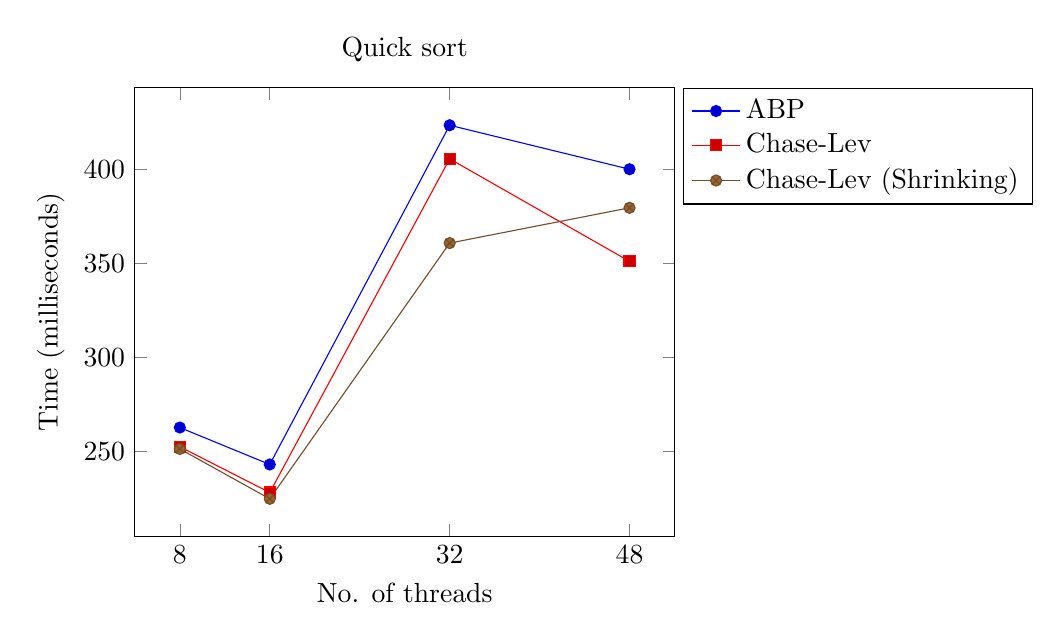
\begin{tikzpicture}
\begin{axis}[
  title={Quick sort},
  xlabel={No. of threads},
  ylabel={Time (milliseconds)},
  xtick={8,16,32,48},
  legend style={at={(1.34,1)}, anchor=north,legend columns=1},
  legend cell align=left
  ]
\addplot+[sharp plot] coordinates % ABP
{(8,262.86) (16,243.2) (32,423.68) (48, 400.28)};
\addplot+[sharp plot] coordinates % Chase-Lev
{(8,252.67) (16,228.27) (32,405.8) (48, 351.26)};
\addplot+[sharp plot] coordinates % Chase-Lev (Shrinking
{(8,251.47) (16,224.93) (32,360.98) (48, 379.75)};
\legend{ABP, Chase-Lev, Chase-Lev (Shrinking)}
\end{axis}
\end{tikzpicture}
\caption{Quick sort scaling.}
\label{fig:qsscaling}
\end{figure}

\subsection{Performance of Idempotent Queues}
Looking at Figure \ref{fig:idemraw}, the idempotent queues are very slow in the raw case. At first this does not seem right as one of the advantages of the idempotent queues should be faster queue operations which is exactly what raw tests. The reason for this bad performance is that there is no synchronization of information on what work is done and what needs to be done. If two threads grab the same task, they both spawn the children of that task, which will be added to their queues. This means that if two workers do the same task it is not only the task itself that has to be executed twice, but also all the children of that task.

\begin{figure}
\begin{tikzpicture}
\begin{axis}[title=Results for 32 threads,  
  ylabel={Relative speedup},
  symbolic x coords={ABP, Idempotent (LIFO), Idempotent (FIFO),
                     Idempotent (Double-ended), Duplicating},
  xtick=data,
  x tick label style={rotate=315,anchor=west},
  legend style={at={(1.17,1)}, anchor=north,legend columns=1},
  legend cell align=left,
  ybar, bar width=10,
  height=150,
  width=300]
\addplot coordinates { % Raw
(ABP,1) (Idempotent (LIFO), 0.210492)
(Idempotent (FIFO), 0.171293) (Idempotent (Double-ended), 0.118589) (Duplicating, 0.708532)
};
\legend{Raw}
\end{axis}
\end{tikzpicture}
\caption{Idempotent performance on raw compared to ABP.}
\label{fig:idemraw}
\end{figure}

This is backed by the fact that the duplicating queue is a lot faster at raw than the other idempotent queues. This is because the duplicating queue only duplicates work when exactly one thief steals a task at the same time as the owner. In the cases of the other idempotent queues it can happen to any number of thieves at the same time, and is therefore a lot more frequently occurring. With less work duplication the duplicating queue performs a lot better in the raw case.
%!TEX root = ../main.tex
\section{Testing}
\label{sec:testing}

%!TEX root = ../Work-stealing Queues.tex
\section{Reflection}
\label{sec:Reflection}
Besides the trouble with testing described in Section~\ref{sec:testing}, we
encountered several problems when trying to perform benchmarks on our various
queue implementations. The most important of these issues are described below.
 
\subsection{Cases For Idempotent Queues}
\label{sub:cases_for_idempotent_queues}
While performing the benchmarks, we realized we had made a mistake when
choosing our cases. First of all, when choosing which cases to implement, we
did not consider which could easily be run with the idempotent queues. This
meant we only had two cases to test the idempotent queues with. Further, the
two cases that happen to work with the idempotent queues are the two cases
that involve the least work for each thread. This makes it hard for us to tell
to which degree the performance of the idempotent queues is effected by queue
operations versus the overhead of possibly performing a piece of work multiple
times.

\subsection{Statistics For Queue Operations}
\label{sub:statistic_for_queue_operations}
Perhaps the greatest issue we found when analyzing our benchmarks, was the lack
of detailed metrics for the queues. For instance, it would be very useful to be
able to measure how many unsuccessful steals occur, and how long each of these
operations take. This degree of detailed information would let us reason more
accurately about the performance characteristics of our different queues and
cases. Unfortunately it is difficult to make these types of measurements
without affecting the execution of the program. If we were only working with
single threaded workloads, the additional overhead from the logging would be
easy to account for. But in our program, where specific interleavings of
multiple threads can produce reasonably large changes in execution time, it is
hard to account for the effects of logging. Regrettably, we did not find an
acceptable solution within the scope of this project.

\subsection{Hardware}
\label{sub:hardware}
One unexpected area where we encountered difficulties was with the processors
on the machine used for benchmarks. For most of the project we were under the
impression that it was a 16 core Intel Xeon processor with hyper-threading.
Later, we found out it had two AMD Opteron processors with 16 cores each.
Strangely, the information in \texttt{/proc/cpuinfo} and the output from
\texttt{lscpu} both implied only 8 physical cores were available on each
processor, with each core exposing two logical cores. To our knowledge, AMD
does not support a technology equivalent to hyper-threading. Because of this,
some uncertainty exists as two how the machine is actually configured.

\subsection{STM-based Queues}
\label{sub:stm_queues}
\todo{Write a bit about STM}

%!TEX root = ../Work-stealing Queues.tex
\section{Conclusion}
\label{sec:conclusion}
% Goal:
% Examine different WSQs
% Expectations
% Chase-Lev good
% Idempotent fast
% Findings
% ABP good
% Idempotent meh



\bibliography{bibliography}

\appendix
%!TEX root = ../../Work-stealing Queues.tex
\section{Run The Project}
\label{app:run}

This project is hosted on Github, at:\\ \url{https://github.com/christianharrington/WorkStealingQueues}
\\
The final revision of the project is: \texttt{493bb55fdd20ced79c7a1e176e2ba3aa3da57dab}

To run the project the Simple Build Tool is required, available from \url{http://www.scala-sbt.org/}, along with a recent version of Java. 
Change directory to \texttt{Scala} inside the repository, and execute \\ \texttt{sbt test} to run the test suite, and \texttt{sbt run} to run the benchmarks.
Various settings relating to the benchmarks can be changed in the settings file, found at: \\ \texttt{Scala/src/main/resources/application.conf}.

%!TEX root = ../../Work-stealing Queues.tex
\section{Results}
\label{app:results}

\begin{figure}
\begin{tikzpicture}
\begin{axis}[title={Results for 8 threads, normalized to ABP},  
  ylabel={Relative speedup},
  symbolic x coords={ABP, Chase-Lev, Chase-Lev (Shrinking), Idempotent (LIFO), Idempotent (FIFO),
                     Idempotent (Double-ended), Duplicating},
  xtick=data,
  x tick label style={rotate=315,anchor=west},
  legend style={at={(1.17,1)}, anchor=north,legend columns=1},
  legend cell align=left,
  ybar, bar width=4,
  height=200,
  width=300]
\addplot coordinates { % Quick sort
(ABP,1) (Chase-Lev, 1.040329) (Chase-Lev (Shrinking), 1.045293) (Idempotent (LIFO), 0)
(Idempotent (FIFO), 0) (Idempotent (Double-ended), 0) (Duplicating, 0)
};
\addplot coordinates { % Spanning tree
(ABP,1) (Chase-Lev, 0.992388) (Chase-Lev (Shrinking), 0.992218) (Idempotent (LIFO), 0.900618)
(Idempotent (FIFO), 1.136076) (Idempotent (Double-ended), 0.900945) (Duplicating, 0.954978)
};
\addplot coordinates { % XML
(ABP,1) (Chase-Lev, 1.413512) (Chase-Lev (Shrinking), 1.427461) (Idempotent (LIFO), 0)
(Idempotent (FIFO), 0) (Idempotent (Double-ended), 0) (Duplicating, 0)
};
\addplot coordinates { % Raw
(ABP,1) (Chase-Lev, 0.620037) (Chase-Lev (Shrinking), 1.087580) (Idempotent (LIFO), 0.260853)
(Idempotent (FIFO), 0.512450) (Idempotent (Double-ended), 0.149191) (Duplicating, 0.679815)
};
\legend{Quick sort, Spanning tree, XML, Raw}
\end{axis}
\end{tikzpicture}
\end{figure}

\begin{figure}
\begin{tikzpicture}
\begin{axis}[title={Results for 16 threads, normalized to ABP},  
  ylabel={Relative speedup},
  symbolic x coords={ABP, Chase-Lev, Chase-Lev (Shrinking), Idempotent (LIFO), Idempotent (FIFO),
                     Idempotent (Double-ended), Duplicating},
  xtick=data,
  x tick label style={rotate=315,anchor=west},
  legend style={at={(1.17,1)}, anchor=north,legend columns=1},
  legend cell align=left,
  ybar, bar width=4,
  height=200,
  width=300]
\addplot coordinates {
(ABP,1) (Chase-Lev, 1.065405) (Chase-Lev (Shrinking), 1.081225) (Idempotent (LIFO), 0)
(Idempotent (FIFO), 0) (Idempotent (Double-ended), 0) (Duplicating, 0)
};
\addplot coordinates {
(ABP,1) (Chase-Lev, 0.948556) (Chase-Lev (Shrinking), 0.949765) (Idempotent (LIFO), 0.770883)
(Idempotent (FIFO), 1.077969) (Idempotent (Double-ended), 0.803096) (Duplicating, 0.924355)
};
\addplot coordinates {
(ABP,1) (Chase-Lev, 1.411119) (Chase-Lev (Shrinking), 1.368644) (Idempotent (LIFO), 0)
(Idempotent (FIFO), 0) (Idempotent (Double-ended), 0) (Duplicating, 0)
};
\addplot coordinates {
(ABP,1) (Chase-Lev, 0.613657) (Chase-Lev (Shrinking), 0.89142) (Idempotent (LIFO), 0.184223)
(Idempotent (FIFO), 0.314387) (Idempotent (Double-ended), 0.109937) (Duplicating, 0.594886)
};
\legend{Quick sort, Spanning tree, XML, Raw}
\end{axis}
\end{tikzpicture}
\end{figure}

\begin{figure}
\begin{tikzpicture}
\begin{axis}[title={Results for 32 threads, normalized to ABP},  
  ylabel={Relative speedup},
  symbolic x coords={ABP, Chase-Lev, Chase-Lev (Shrinking), Idempotent (LIFO), Idempotent (FIFO),
                     Idempotent (Double-ended), Duplicating},
  xtick=data,
  x tick label style={rotate=315,anchor=west},
  legend style={at={(1.17,1)}, anchor=north,legend columns=1},
  legend cell align=left,
  ybar, bar width=4,
  height=200,
  width=300]
\addplot coordinates { % Quick sort
(ABP,1) (Chase-Lev, 1.044061) (Chase-Lev (Shrinking), 1.173693) (Idempotent (LIFO), 0)
(Idempotent (FIFO), 0) (Idempotent (Double-ended), 0) (Duplicating, 0)
};
\addplot coordinates { % Spanning tree
(ABP,1) (Chase-Lev, 1.013258) (Chase-Lev (Shrinking), 1.056889) (Idempotent (LIFO), 0.781902)
(Idempotent (FIFO), 1.191801) (Idempotent (Double-ended), 0.797438) (Duplicating, 0.991763)
};
\addplot coordinates { % XML
(ABP,1) (Chase-Lev, 1.188274) (Chase-Lev (Shrinking), 1.165794) (Idempotent (LIFO), 0)
(Idempotent (FIFO), 0) (Idempotent (Double-ended), 0) (Duplicating, 0)
};
\addplot coordinates { % Raw
(ABP,1) (Chase-Lev, 0.753401) (Chase-Lev (Shrinking), 0.869602) (Idempotent (LIFO), 0.210492)
(Idempotent (FIFO), 0.171293) (Idempotent (Double-ended), 0.118589) (Duplicating, 0.708532)
};
\legend{Quick sort, Spanning tree, XML, Raw}
\end{axis}
\end{tikzpicture}
\end{figure}

\begin{figure}
\begin{tikzpicture}
\begin{axis}[title={Results for 48 threads, normalized to ABP},  
  ylabel={Relative speedup},
  symbolic x coords={ABP, Chase-Lev, Chase-Lev (Shrinking), Idempotent (LIFO), Idempotent (FIFO),
                     Idempotent (Double-ended), Duplicating},
  xtick=data,
  x tick label style={rotate=315,anchor=west},
  legend style={at={(1.17,1)}, anchor=north,legend columns=1},
  legend cell align=left,
  ybar, bar width=4,
  height=200,
  width=300]
\addplot coordinates { % Quick sort
(ABP,1) (Chase-Lev, 1.139554) (Chase-Lev (Shrinking), 1.054061) (Idempotent (LIFO), 0)
(Idempotent (FIFO), 0) (Idempotent (Double-ended), 0) (Duplicating, 0)
};
\addplot coordinates { % Spanning tree
(ABP,1) (Chase-Lev, 0.969213) (Chase-Lev (Shrinking), 1.047708) (Idempotent (LIFO), 0.809070)
(Idempotent (FIFO), 1.153969) (Idempotent (Double-ended), 0.522982) (Duplicating, 0.953984)
};
\addplot coordinates { % XML
(ABP,1) (Chase-Lev, 1.063272) (Chase-Lev (Shrinking), 1.072992) (Idempotent (LIFO), 0)
(Idempotent (FIFO), 0) (Idempotent (Double-ended), 0) (Duplicating, 0)
};
\addplot coordinates { % Raw
(ABP,1) (Chase-Lev, 0.615097) (Chase-Lev (Shrinking), 0.695377) (Idempotent (LIFO), 0.350731)
(Idempotent (FIFO), 0.134826) (Idempotent (Double-ended), 0.140978) (Duplicating, 0.687550)
};
\legend{Quick sort, Spanning tree, XML, Raw}
\end{axis}
\end{tikzpicture}
\end{figure}

\begin{figure}
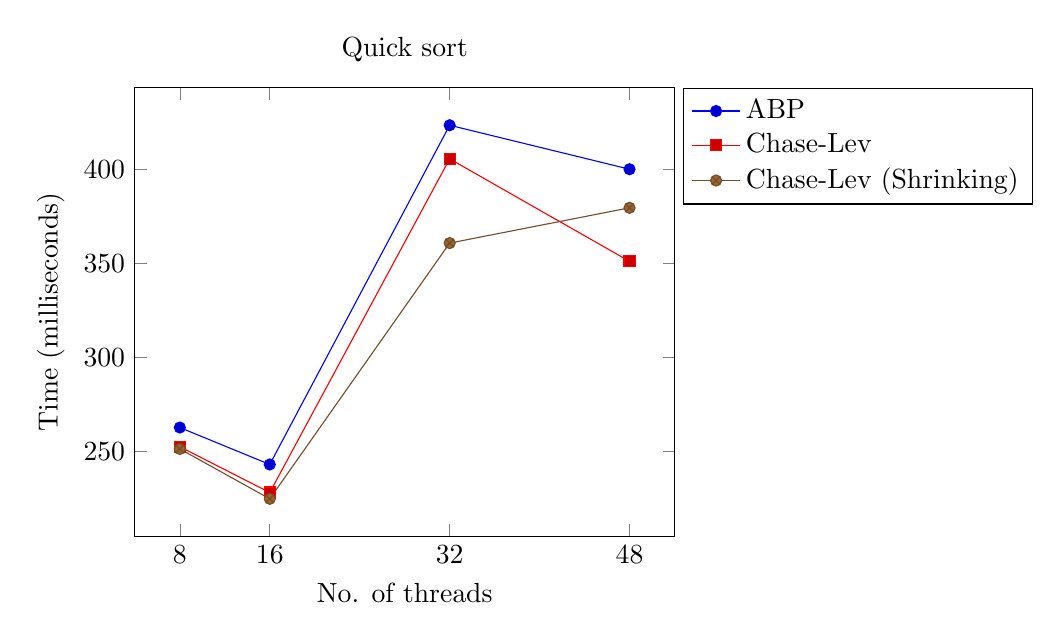
\begin{tikzpicture}
\begin{axis}[
  title={Quick sort},
  xlabel={No. of threads},
  ylabel={Time (milliseconds)},
  xtick={8,16,32,48},
  legend style={at={(1.34,1)}, anchor=north,legend columns=1},
  legend cell align=left
  ]
\addplot+[sharp plot] coordinates % ABP
{(8,262.86) (16,243.2) (32,423.68) (48, 400.28)};
\addplot+[sharp plot] coordinates % Chase-Lev
{(8,252.67) (16,228.27) (32,405.8) (48, 351.26)};
\addplot+[sharp plot] coordinates % Chase-Lev (Shrinking
{(8,251.47) (16,224.93) (32,360.98) (48, 379.75)};
\legend{ABP, Chase-Lev, Chase-Lev (Shrinking)}
\end{axis}
\end{tikzpicture}
\end{figure}

\begin{figure}
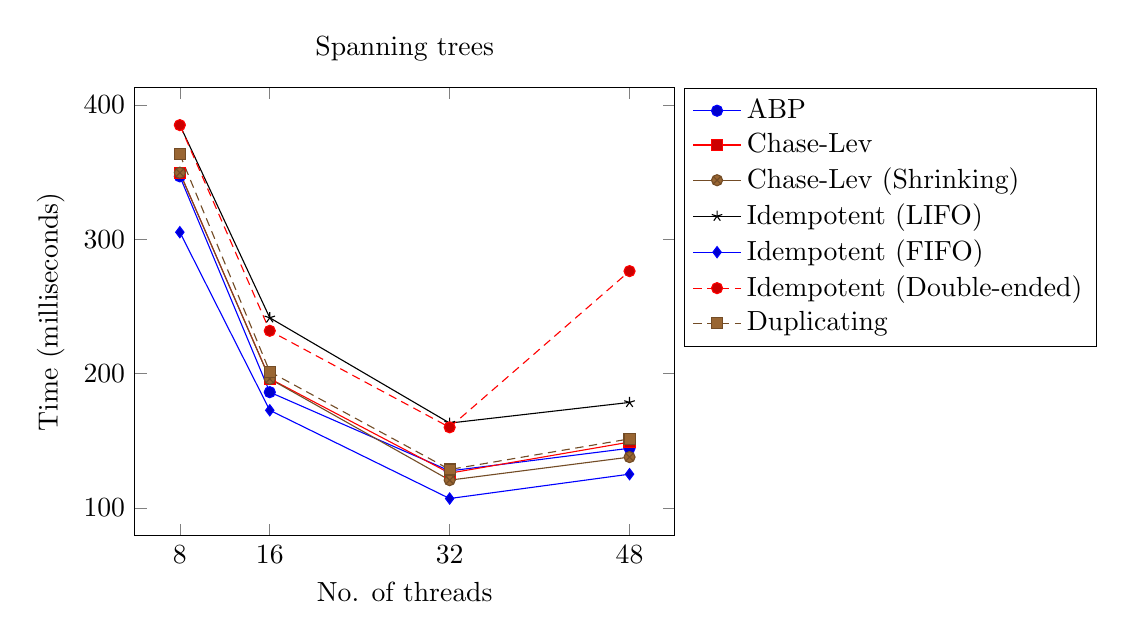
\begin{tikzpicture}
\begin{axis}[
  title={Spanning trees},
  xlabel={No. of threads},
  ylabel={Time (milliseconds)},
  xtick={8,16,32,48},
  legend style={at={(1.4,1)}, anchor=north,legend columns=1},
  legend cell align=left
  ]
\addplot+[sharp plot] coordinates % ABP
{(8,346.81) (16,186.23) (32,127.63) (48, 144.5)};
\addplot+[sharp plot] coordinates % Chase-Lev
{(8,349.47) (16,196.33) (32,125.96) (48, 149.09)};
\addplot+[sharp plot] coordinates % Chase-Lev (Shrinking)
{(8,349.53) (16,196.08) (32,120.76) (48, 137.92)};
\addplot+[sharp plot] coordinates % Idempotent (LIFO)
{(8,385.08) (16,241.58) (32,163.23) (48, 178.6)};
\addplot+[sharp plot] coordinates % Idempotent (FIFO)
{(8,305.27) (16,172.76) (32,107.09) (48, 125.22)};
\addplot+[sharp plot] coordinates % Idempotent (Double-ended)
{(8,384.94) (16,231.89) (32,160.05) (48, 276.3)};
\addplot+[sharp plot] coordinates % Duplicating
{(8,363.15) (16,201.47) (32,128.69) (48, 151.47)};
\legend{ABP, Chase-Lev, Chase-Lev (Shrinking), Idempotent (LIFO), Idempotent (FIFO),
        Idempotent (Double-ended), Duplicating}
\end{axis}
\end{tikzpicture}
\end{figure}

\begin{figure}
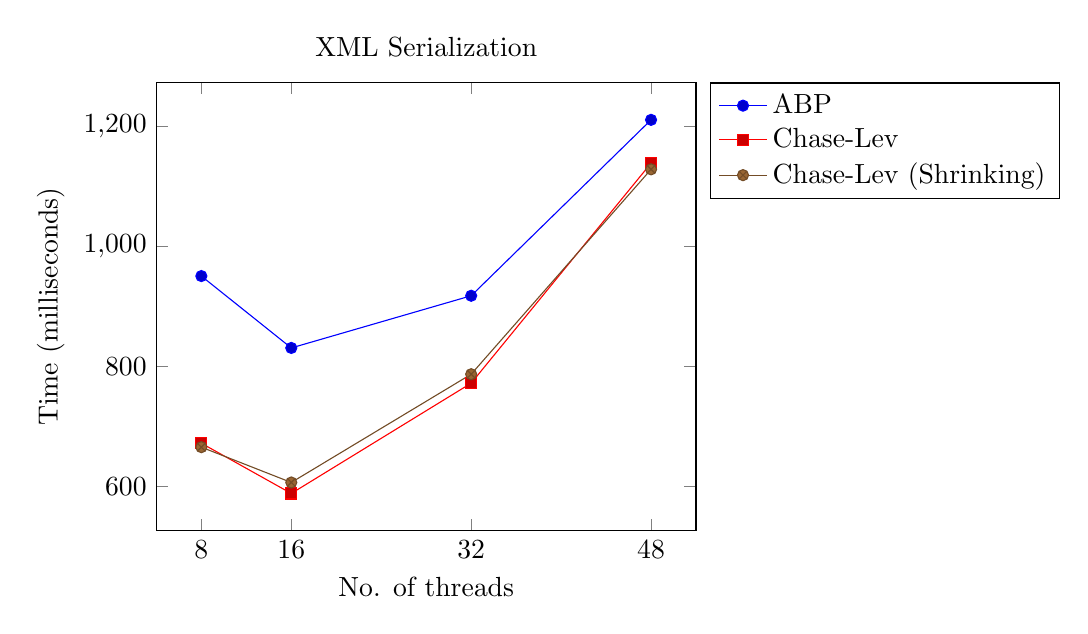
\begin{tikzpicture}
\begin{axis}[
  title={XML Serialization},
  xlabel={No. of threads},
  ylabel={Time (milliseconds)},
  xtick={8,16,32,48},
  legend style={at={(1.35,1)}, anchor=north,legend columns=1},
  legend cell align=left
  ]
\addplot+[sharp plot] coordinates % ABP
{(8,950.29) (16,830.74) (32,917.55) (48, 1210.11)};
\addplot+[sharp plot] coordinates % Chase-Lev
{(8,672.29) (16,588.71) (32,772.17) (48, 1138.10)};
\addplot+[sharp plot] coordinates % Chase-Lev (Shrinking
{(8,665.72) (16,606.98) (32,787.06) (48, 1127.79)};
\legend{ABP, Chase-Lev, Chase-Lev (Shrinking)}
\end{axis}
\end{tikzpicture}
\end{figure}

\begin{figure}
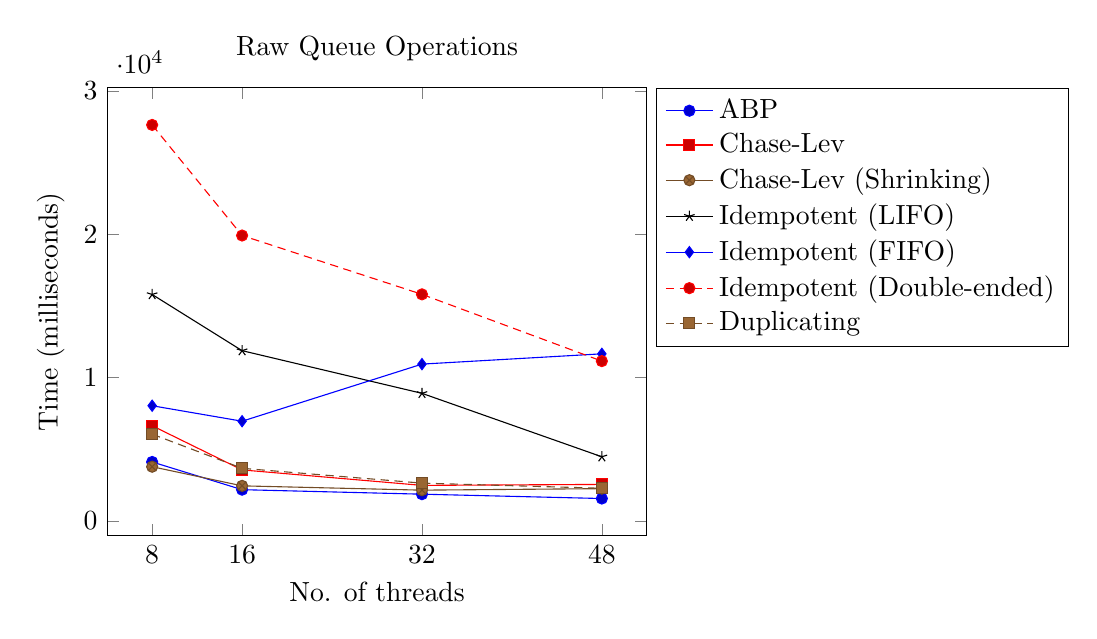
\begin{tikzpicture}
\begin{axis}[
  title={Raw Queue Operations},
  xlabel={No. of threads},
  ylabel={Time (milliseconds)},
  xtick={8,16,32,48},
  legend style={at={(1.4,1)}, anchor=north,legend columns=1},
  legend cell align=left
  ]
\addplot+[sharp plot] coordinates % ABP
{(8,4120.79) (16,2188.83) (32,1874.62) (48, 1572.27)};
\addplot+[sharp plot] coordinates % Chase-Lev
{(8,6646.03) (16,3566.86) (32,2488.21) (48, 2556.13)};
\addplot+[sharp plot] coordinates % Chase-Lev (Shrinking)
{(8,3788.95) (16,2455.44) (32,2155.72) (48, 2261.03)};
\addplot+[sharp plot] coordinates % Idempotent (LIFO)
{(8,15797.32) (16,11881.41) (32,8905.86) (48, 4482.83)};
\addplot+[sharp plot] coordinates % Idempotent (FIFO)
{(8,8041.34) (16,6962.21) (32,10943.90) (48, 11661.40)};
\addplot+[sharp plot] coordinates % Idempotent (Double-ended)
{(8,27620.75) (16,19909.84) (32,15807.66) (48, 11152.57)};
\addplot+[sharp plot] coordinates % Duplicating
{(8,6061.63) (16,3679.41) (32,2645.78) (48, 2286.77)};
\legend{ABP, Chase-Lev, Chase-Lev (Shrinking), Idempotent (LIFO), Idempotent (FIFO),
        Idempotent (Double-ended), Duplicating}
\end{axis}
\end{tikzpicture}
\end{figure}
%!TEX root = ../../Work-stealing Queues.tex
\section{Queue Implementations}
\label{app:queue_impl}
\subsection{ABP Queue}
\begin{lstlisting}[language=scala,basicstyle=\ttfamily\bfseries\scriptsize,numbers=left]
package dk.itu.wsq.queue

import java.util.concurrent.atomic._

case class Tag(val value: Int) extends AnyVal

class ABPQueue[E](val size: Int) extends WorkStealingQueue[E] {
  case class Age(val tag: Tag, val top: Int) {
    override def equals(that: Any) = that match {
      case t: Age => tag == t.tag && top == t.top
      case _      => false
    }
  }

  private val age = new AtomicReference[Age](Age(Tag(0), 0))
  private var bottom: Int = 0
  private val queue = new AtomicReferenceArray[E](size)

  final def push(v: E): Unit = {
    val localBot = bottom
    queue.set(localBot, v)
    bottom = localBot + 1
  }

  final def take(): Option[E] = {
    val oldBottom = bottom

    if (oldBottom == 0) {
      None
    }
    else {
      val localBot = oldBottom - 1
      bottom = localBot

      val v = queue.get(localBot)
      val oldAge = age.get
      
      if (localBot > oldAge.top) {
        Some(v)
      }
      else {
        bottom = 0
        val newAge = new Age(Tag(oldAge.tag.value + 1), 0)
        if (localBot == oldAge.top) {
          if (age.compareAndSet(oldAge, newAge)) {
            Some(v)
          }
          else {
            age.set(newAge)
            None
          }
        }
        else {
          age.set(newAge)
          None
        }
      }
    }
  }

  final def steal(): Option[E] = {
    val oldAge = age.get
    val localBot = bottom

    if (localBot <= oldAge.top) {
      None
    }
    else {
      val v = queue.get(oldAge.top)
      val newAge = Age(oldAge.tag, oldAge.top + 1)

      if (age.compareAndSet(oldAge, newAge)) {
        Some(v)
      }
      else {
        None
      }
    }
  }

  final def length = bottom - age.get.top
}
\end{lstlisting}

\subsection{Chase-Lev Queue (Both Versions)}
\begin{lstlisting}[language=scala,basicstyle=\ttfamily\bfseries\scriptsize,numbers=left]
package dk.itu.wsq.queue

class CircularArray[E: Manifest](val logSize: Int) {
  // Initial size = 2^logSize
  private val segment: Array[E] = new Array[E](1 << logSize)

  def size: Long = 1 << logSize

  def apply(index: Long): E = get(index)

  def update(index: Long, element: E) = put(index, element)

  def get(index: Long): E = {
    segment((index % size).toInt)
    // TODO: Improve this by using a bit mask
  }

  def put(index: Long, element: E): Unit = {
    segment((index % size).toInt) = element
    // TODO: Improve this by using a bit mask
  }

  def grow(bottom: Long, top: Long): CircularArray[E] = {
    val newArray = new CircularArray(logSize + 1)
    var i = top
    for (i <- top until bottom) {
      newArray(i) = get(i)
    }

    newArray
  }

  def shrinkNaive(bottom: Long, top: Long): CircularArray[E] = {
    val newArray = new CircularArray(logSize - 1)
    var i = top
    for (i <- top until bottom) {
      newArray(i) = get(i)
    }

    newArray    
  }
  
}

class ChaseLevQueue[E: Manifest] extends WorkStealingQueue[E] {
  import java.util.concurrent.atomic._
  
  // Never decremented. Assumed to never overflow.
  protected var top: AtomicLong = new AtomicLong(0)
  // Indicates where next element is pushed
  @volatile protected var bottom: Long = 0
  
  // Initial size is 2^logInitialSize
  protected val logInitialSize = 2
  @volatile protected var activeArray = new CircularArray[E](logInitialSize)

  final def push(element: E): Unit = {
    val b = bottom
    val t = top.get
    var arr = activeArray
    val size = b - t
    // If the array is too small, grow the array
    if (size >= arr.size - 1) {
      arr = arr.grow(b, t)
      activeArray = arr
    }

    arr(b) = element
    bottom = b + 1
  }

  final def steal(): Option[E] = {
    val t = top.get
    val b = bottom
    val arr = activeArray
    val size = b - t

    if (size <= 0) {
      None
    } else {
      val elem = arr(t) // Get top element

      if (top.compareAndSet(t, t + 1)) 
        Some(elem)
      else 
        None
    }
  }

  def take(): Option[E] = {
    var b = bottom
    val arr = activeArray
    b = b - 1
    bottom = b
    val t = top.get
    val size = b - t

    if (size < 0) {
      bottom = t
      None
    } else {
      val elem = arr(b) // Get bottom element

      if (size > 0) {
        Some(elem)
      } else {
        bottom = t + 1
        if (top.compareAndSet(t, t + 1)) 
          Some(elem) 
        else
          None
      }
    }
  }

  final def length = (bottom - top.get).toInt
}
\end{lstlisting}

\subsection{Idempotent LIFO Queue}
\begin{lstlisting}[language=scala,basicstyle=\ttfamily\bfseries\scriptsize,numbers=left]
package dk.itu.wsq.queue

class IdempotentLIFO[E: Manifest] extends WorkStealingQueue[E] {
  import java.util.concurrent.atomic._
  import scala.annotation.tailrec

  case class Anchor(tail: Int, tag: Int)

  private val anchor: AtomicReference[Anchor] = 
  		new AtomicReference[Anchor](Anchor(0, 0)) // (tail, tag)
  private var capacity: Int = 1
  private var tasks: Array[E] = new Array[E](capacity)

  @tailrec
	final def push(e: E): Unit = {    
    val localAnchor = anchor.get()

    if(localAnchor.tail == capacity) {
      // Capacity limit reached, expand and try again
      expand() 
      push(e)
    } else {
      // Else put the element and write to anchor with read values plus one
      tasks(localAnchor.tail) = e
      anchor.set(Anchor(localAnchor.tail + 1, localAnchor.tag + 1))
    }
  }

	final def take(): Option[E] = {    
    val localAnchor = anchor.get()

    if(localAnchor.tail == 0) {
      None
    } else {
      val task = tasks(localAnchor.tail - 1)
      anchor.set(Anchor(localAnchor.tail - 1, localAnchor.tag))
      Some(task)
    }
  }

  @tailrec
  final def steal(): Option[E] = {
    val localAnchor = anchor.get()
    if(localAnchor.tail == 0) {
      None
    } else {
      val arr = tasks
      val task = arr(localAnchor.tail - 1)
      if(anchor.compareAndSet(localAnchor, Anchor(localAnchor.tail - 1, localAnchor.tag))) {
        Some(task)
      }
      else {
        steal()
      }
    }
  }

  final private def expand(): Unit = {
    val newCapacity = capacity * 2
    val arr = new Array[E](newCapacity)

    for(i <- 0 until capacity) { arr(i) = tasks(i) }

    tasks = arr
    capacity = newCapacity
  }

  final def length: Int = anchor.get().tail
}
\end{lstlisting}

\subsection{Idempotent FIFO Queue}
\begin{lstlisting}[language=scala,basicstyle=\ttfamily\bfseries\scriptsize,numbers=left]
package dk.itu.wsq.queue

class IdempotentFIFO[E: Manifest] extends WorkStealingQueue[E] {
  import java.util.concurrent.atomic._
  import scala.annotation.tailrec

  private val head: AtomicInteger = new AtomicInteger(0)
  private var tail: Int = 0
  private var tasks: Array[E] = new Array[E](1)

  @tailrec
	final def push(e: E): Unit = {
    val h = head.get()
    val t = tail
    if(t >= h + tasks.length) {
      expand()
      push(e)
    } else {
      tasks(t % tasks.length) = e
      tail = t + 1 
    }
  }

	final def take(): Option[E] = {
    val h = head.get()
    val t = tail
    if(h == t) {
      None
    } else {
      val task = tasks(h % tasks.length)
      head.set(h + 1)
      Some(task)
    }
  }

  @tailrec
  final def steal(): Option[E] = {
    //println("Stealing...")
    val h = head.get()
    val t = tail
    if(h == t) {
      None
    } else {
      val arr = tasks
      val task = arr(h % arr.length)
      if(head.compareAndSet(h, h + 1)) {
        Some(task)
      }
      else {
        steal()
      }
    }
  }

  private final def expand(): Unit = {
    val size = tasks.length
    val arr = new Array[E](size * 2)
    for (i <- head.get() until tail) {
      arr(i % arr.length) = tasks(i % tasks.length)
    }
    tasks = arr
  }

  final def length: Int = tail - head.get()
}

\end{lstlisting}

\subsection{Idempotent Double-Ended Queue}
\begin{lstlisting}[language=scala,basicstyle=\ttfamily\bfseries\scriptsize,numbers=left]
package dk.itu.wsq.queue

class IdempotentDE[E: Manifest] extends WorkStealingQueue[E] {
  import java.util.concurrent.atomic._
  import scala.annotation.tailrec

  case class Anchor(head: Int, size: Int, tag: Int)

  @volatile private var tasks: Array[E] = new Array[E](1)

  @volatile private var anchor: AtomicReference[Anchor] = 
    new AtomicReference[Anchor](Anchor(0, 0, 0)) // (head, size, tag)

  @tailrec
  final def push(e: E): Unit = {
    val localAnchor = anchor.get()
    if (localAnchor.size == tasks.length) {
      expand()
      push(e)
    } else {
      tasks((localAnchor.head + localAnchor.size) % tasks.length) = e
      anchor.set(Anchor(localAnchor.head, localAnchor.size + 1, localAnchor.tag + 1))
    }
  }

  final def take(): Option[E] = {
    val localAnchor = anchor.get()
    if (localAnchor.size == 0) {
      None
    } else {
      val task = tasks((localAnchor.head + localAnchor.size - 1) % tasks.length)
      anchor.set(Anchor(localAnchor.head, localAnchor.size - 1, localAnchor.tag))
      Some(task)
    }
  }

  @tailrec
  final def steal(): Option[E] = {
    val localAnchor = anchor.get()
    if (localAnchor.size == 0) {
      None
    } else {
      val arr = tasks.clone()
      val task = arr(localAnchor.head % arr.length)
      if (anchor.compareAndSet(
      	localAnchor, Anchor(localAnchor.head + 1, localAnchor.size - 1, localAnchor.tag)
      	)) {
        Some(task)
      }
      else {
        steal()
      }
    }
  }

  final def expand(): Unit = {
    val localAnchor = anchor.get()
    val arr = new Array[E](localAnchor.size * 2)
    for (i <- 0 until localAnchor.size) {
      arr((localAnchor.head + i) % arr.length) = tasks((localAnchor.head + i) % tasks.length)
    }
    tasks = arr
  }

  final def length: Int = anchor.get().size
}

\end{lstlisting}

\subsection{Duplicating Queue}
\begin{lstlisting}[language=scala,basicstyle=\ttfamily\bfseries\scriptsize,numbers=left]
package dk.itu.wsq.queue

class DuplicatingQueue[E: Manifest](val size: Int) extends WorkStealingQueue[E] {
  import scala.annotation.tailrec

  private val tasks: Array[Option[E]] = new Array[Option[E]](size)
  @volatile private var head: Int = 0
  @volatile private var tail: Int = 0
  private var tailMin = Integer.MAX_VALUE

  @tailrec
  final def push(e: E): Unit = {
    if(tail < (Math.min(tailMin, head) + size) && tail < Integer.MAX_VALUE/2) {
      tasks(tail % size) = Some(e)
      tail += 1
    } else {
      this.synchronized {
        if(head > tailMin) {
          head = tailMin
        }
        tailMin = Integer.MAX_VALUE

        val count = Math.max(0, tail - head)

        head = head % size
        tail = tail + count
      }
      push(e) // In the paper they run the task here.
    }
  }

  final def take(): Option[E] = {
    tail -= 1
    if(head <= Math.min(tailMin, tail)) {
      if(tailMin > tail) {
        tailMin = tail
      }      
      val task = tasks(tail % size)
      tasks(tail % size) = None
      task
    } else {
      this.synchronized {
        if(head > tailMin) {
          head = tailMin
        }
        tailMin = Integer.MAX_VALUE
        if(head <= tail) {
          val task = tasks(tail % size)
          tasks(tail % size) = None
          task
        } else {
          tail += 1
          None
        }
      } 
    }
  }

  final def steal(): Option[E] = {
    this.synchronized {
      if(head < tail) {
        val task = tasks(head % size)
        head += 1
        task
      } else {
        None
      }
    }
  }

  final def length: Int = tail - head
}

\end{lstlisting}



\end{document}